% =========================================================
% CONFIGURACION DEL DOCUMENTO
% =========================================================
\providecommand{\main}{..}
\documentclass[\main/main.tex]{subfiles}

% =========================================================
% CONTENIDO
% =========================================================
\begin{document}
\chapter{Sistema propuesto}
\label{cha:03_sistema_propuesto}
	% ===============================================================
	% ===============================================================
	\section{\textit{Setup} a utilizar}
	\label{sec:03_setup}
		Debido a que este trabajo de memoria corresponde fundamentalmente a una prueba de concepto se decidió junto al profesor guía evitar en lo posible la compra de nuevo equipamiento y por tanto no se entrega particular importancia a cumplir de forma estricta con las características de hardware utilizado en instancias formales de investigación. Con esto en consideración se presenta a continuación una descripción del entorno de hardware y software utilizado:
		\begin{table}[H]\begin{center}\footnotesize{
			\singlespacing{
			\begin{tabular}{| C{0.11\textwidth} | C{0.14\textwidth} | R{0.18\textwidth} L{0.5\textwidth} |} \hline
				\multirow{8}{*}{Hardware} 	& \multirow{4}{*}{PC} 			& Procesador: 		& Intel Core i7-3770 \\
										& 							& Memoria RAM:		& $16.0[GB]$, DDR3, $650[MHz]$ \\
										& 							& Disco duro: 		& Samsung SSD, 840 Series, $120[GB]$ \\
										& 							& Tarjeta gráfica: 	& NVIDIA GeForce GTX 660 Ti, $2[GB]$ \\ \cline{2-4}
										& \multirow{2}{*}{Monitores}& Principal:		& Samsung SyncMaster, $1680\times1050[px]$, $60[Hz]$ \\ 
										& 							& Secundario: 		& Samsung SyncMaster, $1680\times1050[px]$, $60[Hz]$ \\ \cline{2-4} 
										& Adquisición 				& \textit{Eye tracker}: 		& EyeTribe \\ \cline{2-4}
										& Otro 						& Apoya-barbilla: 	& Diseñado y contruido en la universidad\footnotemark. \\ \hline
				\multirow{4}{*}{Software} 	& \multirow{2}{*}{Entorno} 		& SO:				& Windows 10 Pro x64 \\ 
										& 							& Base:				& Python 2.7 x86, Anaconda \\ \cline{2-4}
										& \multirow{2}{*}{Módulos}		& Principal: 			& PsychoPy 1.84.2\cite{psychopy} \\
										& 							& Requeridos:			& Ver anexo \ref{cha:a01_instalacion} \\ \hline
			\end{tabular}}
			\caption{Hardware y software utilizado en el desarrollo.}
			\label{tbl:03_hs_selection}
		}\end{center}\end{table}
		\footnotetext{Diseñado y construido por Christopher Rozas con colaboración del departamento de IDP de la Universidad Técnica Federico Santa María.}

		\newpage
		La elección de software se encuentra infuenciada fuertemente por los siguientes puntos:
		\begin{enumerate}\setlength\itemsep{-0.5em}
			\item El \textit{eye tracker} a utilizar solo tiene disponible sus drivers para Mac y Windows. Debido a la facilidad de encontrar computadoras con Windows se decanta por este \acrshort{so}.

			\item Los desafíos del sistema a implementar requieren del uso de un lenguaje orientado a objetos. A pesar de las bondades de Octave o Matlab en procesamiento y acceso a módulos complementarios estos entornos carecen de buen soporte para este tipo de programación, por este motivo se utiliza Python como lenguaje de desarrollo. 

			\item Dentro de las opciones disponibles PsychoPy resulta sumamente interesante. Cumple con ser open-source, es ampliamente utilizado por investigadores, presenta documentación detallada y clara para todas sus funciones y los foros se encuentran activos. Otro punto interesante es que entrega soporte para varias marcas de \textit{eye tracker}, entre los cuales se encentra el seleccionado.

		\end{enumerate}

	% ===============================================================
	% ===============================================================
	\section{Diseño del sistema}
	\label{sec:03_diseño_sistema}
		El sistema a ser desarrollado en este trabajo de título tiene como función principal facilitar el proceso de configuración y puesta en marcha de experimentos asociados a movimiento ocular. Para esto, se considera oportuno subdividir el desarrollo en tres partes: La primera consiste en determinar la estructura de datos requerida para almacenar tanto las configuraciones del sistema como de las tareas a implementar. La segunda implica la implementación de los métodos de configuración y ejecución del experimento, asegurando su correcto funcionamiento. La tercera etapa corresponde a montar estas funciones en una GUI para facilitar el proceso a personas que no tengan conocimiento del lenguaje. Así, se presenta a continuación el trabajo realizado.

		% ###########################################################
		\subsection{Primera parte: Estructura de datos}
		\label{sub:03_estructura_datos}
			Al diseñar la estructura de datos se debió considerar el problema desde tres aristas. La primera correspondía a la necesidad de almacenar la información del conjunto compuesto por experimento-tareas-cuadros-componentes donde, complementando lo expuesto en el apartado \ref{sub:02_experimentos_de_estimulacion}, las tareas corresponden a las actividades específicas que el paciente debe reaizar. Los cuadros corresponden a los elementos que conforman dichas tareas y los componentes serán considerados como las figuras e imágenes contenidas en cada cuadro. La segunda dice relación con la información complementaria que se desea incluir para posterior análisis, tal como comentarios del investigador encargado del experimento para una sesión específica o algunas características de quien realizará el experimento, tales como su edad, sexo, color de ojos o si se utilizan lentes durante la ejecución. Finalmente, la tercera arista implica el conservar las configuraciones del equipo y hardware a utilizar para montar el servicio de ejecución asociado al módulo ioHub, que es el componente de PsychoPy que permite sincronizar todos los dispositivos asociados a la ejecución del experimento: teclado, pantalla, \textit{eye tracker}, etc. y almacenar los datos en un archivo. 
			\begin{figure}[H]
				\centering
				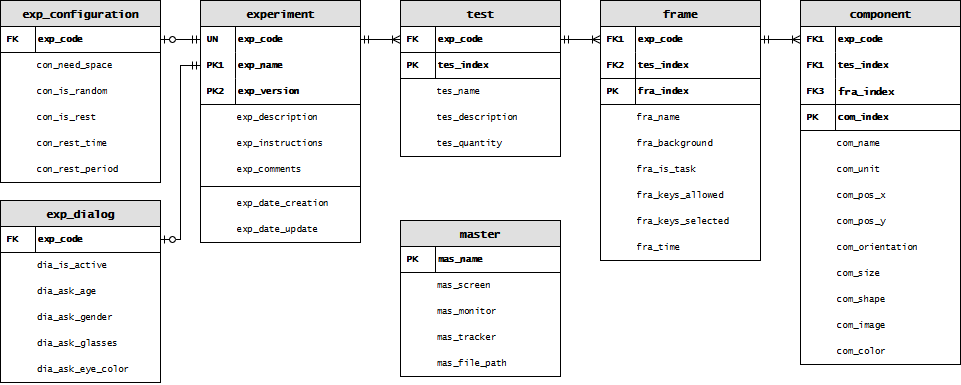
\includegraphics[width=\textwidth]{cap_03_database}
				\caption{Diagrama de base de datos a implementar.}
				\label{fig:03_database}
			\end{figure} 

			En base a lo anterior, se propone como solución el uso de una base de datos local de tipo \textit{SQLite} con la estructura presentada en la figura \ref{fig:03_database}. A continuación se comenta el contenido de cada tabla propuesta y su función:
			\begin{enumerate}\setlength\itemsep{-0.5em}
				\item \textbf{\textref{configuration}:} Almacena la información asociada a un perfil de configuración. Cada perfil se identifica con un nombre (\textref{con\_name}) e indica qué monitor será utilizado (\textref{con\_screen}), cuál es su configuración\footnote{Los parámetros del monitor se definen en un aplicativo especializado de \textit{psychoPy}.} (\textref{con\_monitor}), el \textit{eye tracker} a utilizar (\textref{con\_tracker}) y el directorio en que serán almacenados los resultados (\textref{con\_path}).

				\item \textbf{\textref{experiment}:} Almacena la configuración de un experimento. Cada experimento se identifica por un código único (\textref{exp\_code}) y un par nombre / versión (\textref{exp\_name} / \textref{exp\_version}), que tiene como objetivo identificar a una aplicación específica de una familia del mismo tipo, por ejemplo: (''antisaccade'' / ''v1.0''). Además, se incluye un campo para indicar una descripción (\textref{exp\_description}), instrucciones para el usuario (\textref{exp\_instructions}) y comentarios para quien tome el experimento (\textref{exp\_comments}). Se incluyen la fecha de creación y la última modificación para dejar de forma explícita una señal de cuidado: Las condiciones del experimento pueden no ser las mismas de la última ejecución.
				
				\item \textbf{\textref{exp\_configuration}:} Esta tabla es complementaria al experimento y almacena la configuración general de ejecución. \textquestiondown Es necesario que el paciente presione la tecla espacio antes de cada tarea? (\textref{exp\_need\_space}), \textquestiondown El orden de las tareas es aleatorio o secuencial? (\textref{exp\_is\_random}), \textquestiondown Se incluyen en el experimento tiempos de descanso? (\textref{exp\_is\_rest}), \textquestiondown Cada cuántas tareas? (\textref{exp\_rest\_period}), \textquestiondown Con qué duración? (\textref{exp\_rest\_time}).

				\item \textbf{\textref{exp\_dialog}:} Esta tabla es complementaria al experimento y almacena la configuración del diálogo inicial, que permite obtener información adicional sobre el paciente. \textquestiondown Es necesario incluir información complementaria? (\textref{dia\_is\_active}), \textquestiondown Qué edad tiene el paciente? (\textref{dia\_ask\_age}), \textquestiondown Cuál es su sexo? (\textref{dia\_ask\_gender}), \textquestiondown Utiliza gafas o lentes de contacto? (\textref{dia\_ask\_glasses}), \textquestiondown Cuál es su color de ojos? (\textref{dia\_ask\_eye\_color}).

				\item \textbf{\textref{test}:} Almacena, para cada experimento, la identificación de las tareas que lo componen ordenadas por un índice (\textref{tes\_index}). Cada tarea se identifica por su nombre (\textref{tes\_name}), que es único para cada experimento, y un campo para añadir su descripción (\textref{tes\_description}).

				\item \textbf{\textref{exp\_sequence}:} Almacena, para cada experimento, la secuencia de tareas a ejecutar. Cada ítem incluye un identificador del experimento (\textref{exp\_code}) y la tarea correspondiente (\textref{tes\_index}), además de un índice que permite definir el orden de ejecución (\textref{seq\_index}) y el número de veces que debe ejecutarse la tarea (\textref{seq\_quantity}). 

				\item \textbf{\textref{frame}:} Esta tabla contiene, para cada tarea, el conjunto de cuadros que la conforman ordenados por aparición mediante un índice (\textref{fra\_index}). Cada cuadro se identifica por un nombre (\textref{fra\_name}),  único para cada tarea, y permite la configuración de su comportamiento y características de forma general: color de fondo (\textref{fra\_color}), si el cuadro corresponde a una tarea que requiere respuesta de teclado o es temporizada (\textref{fra\_is\_task}), las teclas habilitadas (\textref{fra\_keys\_allowed}) y las teclas que se espera sean presionadas (\textref{fra\_keys\_correct}) en el primer caso o el tiempo por el cual debe ser presentado (\textref{fra\_time}) en el segundo.

				\item \textbf{\textref{component}:} Esta tabla contiene, para cada cuadro, el conjunto de componentes o elementos que lo conforman ordenados por presentación mediante un índice (\textref{com\_index}). Cada componente se identifica por un nombre (\textref{com\_name}), único para cada cuadro, y las configuraciones asociadas tanto a las unidades de medida a utilizar (\textref{com\_units}), su posición en la pantalla ((\textref{com\_pos\_x}), (\textref{com\_pos\_y})), su tamaño (\textref{com\_size}), si se encuentra rotada o no (\textref{com\_rotation}), en el cao de ser figura su forma (\textref{com\_shape}) y color (\textref{com\_color}) o si es una imagen la información binaria correspondiente (\textref{com\_image}). 
			\end{enumerate}

			Este modelo se considera apropiado por los siguientes motivos:
			\begin{enumerate}\setlength\itemsep{-0.5em}
				\item Aísla un experimento de otro al tener tareas y configuraciones completamente independientes. Esta configuración permite evitar que cambios en alguna tarea específicas afecte a mas de un experimento.

				\item No puede existir una tarea que no se encuentre asociada a un experimento, lo que evita almacenar datos innecesarios (esto aplica también a cuadros y componentes). 

				\item Tener todas las configuraciones almacenadas en un archivo facilita la portabilidad y migración desde un equipo a otro. Además, dado que es tratable como una base de datos convencional facilita el proceso de revisión de los datos sin necesidad de contar con el programa principal.
			\end{enumerate}

			Cabe destacar que, para asegurar la limpieza de la base de datos se tomo la decisión de definir las operaciones de \textit{update} como \textit{delete} en cascada a todas las tablas asociadas a un experimento. Esto implica que al eliminar un experimento particular se eliminan todos los datos dependientes de él, tales como sus tareas, cuadros y componentes, evitando mantener data residual. Cabe destacar que esto se define también en niveles más bajos: eliminar una tarea elimina todos sus cuadros, eliminar un cuadro elimina también todos sus componentes.  

		% ###########################################################
		\subsection{Segunda parte: Implementación de las funciones principales}
		\label{sub:03_implementacion_backtend}
			Para lograr sincronizar la ejecución del experimento con el uso de dispositivos tales como el monitor, teclado y \textit{eye tracker} se hará uso de \textit{ioHub} \cite{website:iohub}. Esta herramienta, que forma parte de los módulos de \textit{psychoPy}, tiene por característica principal la capacidad de montar un servicio que permite ralizar una revisión constante de los dispositivos de entrada/salida configurados previamente para el experimento, almacenando la información recopilada de forma ordenada en un archivo con formato \textit{hdf5}. Este tipo de archivos es considerado estándar en investigación y, a grandes rasgos, corresponde a un tipo \textit{\gls{log}} de datos organizado a modo de diccionario. Utilizando esta aplicación se plantea formular un sistema que permita las funcionalidades presentadas en la figura \ref{fig:03_application_concept}. 
			\begin{figure}[H]
				\centering
				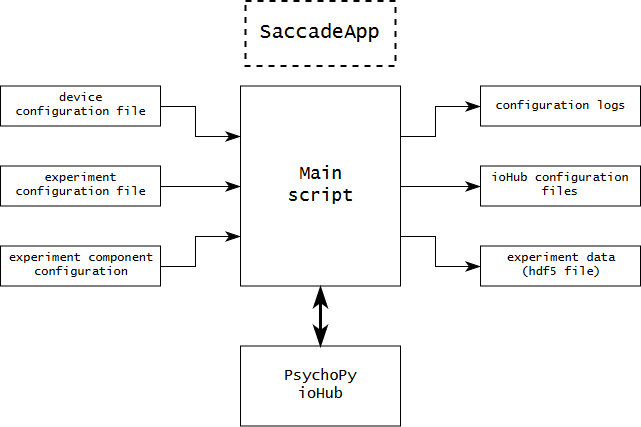
\includegraphics[width=0.8\textwidth]{cap_03_application_concept}
				\caption{Diagrama de funcionamiento general.}
				\label{fig:03_application_concept}
			\end{figure} 

			La aplicación propuesta tiene por requerimientos tanto la configuración del experimento (\textref{Experiment}) como la del perfil de configuración (\textref{Configuration Profile}), explicados en la sección \ref{sub:03_estructura_datos}.

			Los resultados esperados son:
			\begin{enumerate}\setlength\itemsep{-0.5em}
				\item Creación de una estructura de carpetas que permita almacenar la información de las distintas instancias de ejecución de forma organizada y clara. 

				Para lograr esto se propone el sistema de la figura \ref{fig:03_folder_structure} que consiste en separar los resultados por tipo de experimento y por versión. De esta forma, en el directorio base determinado en el perfil de configuración (\textref{Base\_Folder}) se crean carpetas con los nombres de los experimentos ejecutados (\textref{Experiment\_Name}) y dentro de estas se organizan los resultados en carpetas que indican la versión del experimento (\textref{Experiment\_Version}) y su código (\textref{Experiment\_Code}).  
				\begin{figure}[H]
					\centering
					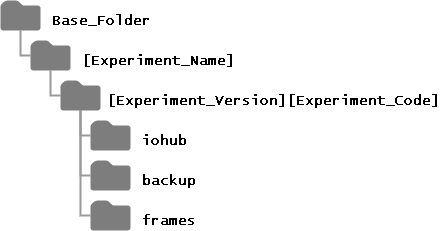
\includegraphics[width=0.6\textwidth]{cap_03_folder_structure}
					\caption{Estructura de directorios para resultados.}
					\label{fig:03_folder_structure}
				\end{figure} 

				\item Para facilitar el proceso de revisión y posterior \textit{debug} de los experimentos realizados se decide almacenar en la carpeta de resultados 3 archivos: El primer archivo, a almacenar en la carpeta \textref{backup} consiste en un diccionario que contiene todas las configuraciones asociadas al experimento y perfil utilizados (\textref{Backup Configuration File}). Los siguientes 2 archivos, a almacenar en la carpeta \textref{ioHub}, corresponden a las configuraciones del experimento y hardware en el formato requerido por \textit{ioHub} para su funcionamiento (\textref{ioHub Configuration Files}). Para identificar una ejecución de otra, cada grupo de archivos se identifica por la marca de tiempo del momento de ejecución en formato \textit{Unix}.

				\item Los resultados del experimento (\textref{Experiment Data}) se almacenan directamente en la carpeta \textref{[Experiment\_Version][Experiment\_Code]}. Este archivo se actualiza con cada ejecución y contiene los resultados de todas las sesiones del experimento. 

				\item De forma opcional, el \textit{script} permite obtener capturas de pantalla de cada uno de los cuadros del experimento (\textref{Frame Images}). Estas imagenes son almacenadas en la carpeta \textref{frames}. 
			\end{enumerate}

			En la figura \ref{fig:03_base_class_tree} se presenta la estructura de clases implementada en este trabajo de título. Las clases \textref{Configuration}, \textref{Experiment}, \textref{Test}, \textref{Frame} y \textref{Component} representan el conjunto de métodos que permiten la manipulación de los datos almacenados en la base de datos, además de entregar funcionalidades que permiten la ejecución. 
			\begin{figure}[H]
				\centering
				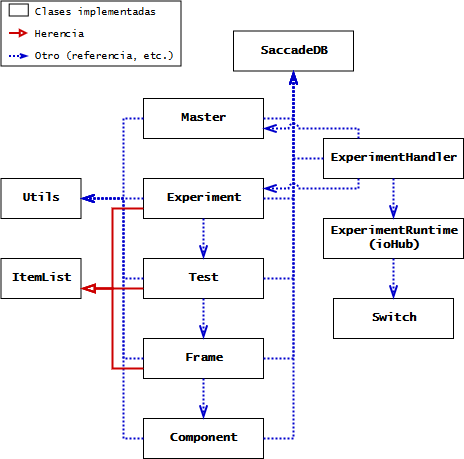
\includegraphics[width=\textwidth]{cap_03_base_class_tree}
				\caption{Diagrama de clases del sistema (no considera GUI).}
				\label{fig:03_base_class_tree}
			\end{figure} 

			Debido a que las clases \textref{Experiment}, \textref{Test} y \textref{Frame} implican el manejo de una lista de objetos se crea una clase base llamada \textref{ItemList} que permite integrar funcionalidades tales como agregar, quitar, mover o reemplazar elementos. Además, ya que un experimento implica la ejecución de una secuencia de tareas que pueden repetirse se implementa una variante de \textref{ItemList} que permite la manipulación de secuencias en base a los elementos disponibles en lista \textref{ItemListSequence}.

			Las clases \textref{SaccadeDB} y \textref{Switch} añaden funcionalidades transversales al resto de las clases: \textref{SaccadeDB} permite la comunicación e interacción con el archivo de base de datos y \textref{Switch} permite implementar estructuras \textit{switch-case} para facilitar el uso de máquinas de estado. \textref{ExperimentHandler} y \textref{ExperimentRuntime} (que hereda sus funcionalidades de \textref{ioHub} e inicializa los servicios asociados) son las encargadas de preparar los archivos de configuración y ejecutar el experimento respectivamente.   

			En las siguientes páginas se procede a describir con un mayor grado de detalle cada clase y módulo utilizado. Por simplicidad se obvian las funciones asociadas al get-set de los atributos de las clases (ya que corresponden a los datos almacenados en la base de datos).
			
			\newpage
			\begin{enumerate}\setlength\itemsep{-0.5em}
				\item \textbf{\textref{utils}:} Módulo auxiliar que implementa métodos de uso general.
				
				\vspace{-8mm}			
				\begin{center}\footnotesize{\singlespacing{
					\begin{longtable}[H]{| C{0.15\textwidth} | R{0.13\textwidth} L{0.6\textwidth} |} \hline
						% ===============================================
						\multicolumn{3}{|c|}{\multirow{2}{*}{\textref{format\_text}}}\\\multicolumn{3}{|c|}{}\\\hline
						Descripción & \multicolumn{2}{L{0.75\textwidth}|}{
						Convierte el dato de entrada a unicode. Si el dato ingresado no cumple con las condiciones de formato se levanta una excepción indicando el error asociado.
						}\\\hline
						\multirow{4}{*}{Inputs} & text: 		& Dato a ser convertido en unicode. \\
						 						& lmin: 		& Largo mínimo (int). Por defecto: None (Sin condición). \\
						 						& lmax: 		& Largo máximo (int). Por defecto: None (Sin condición)\\
						 						& var\_name:	& Nombre de la variable para la cual se utilizará el dato formateado (string). Se agrega en el mensaje de excepción para hacer seguimiento del error. Por defecto: vacío (Sin nombre).
						\\\hline
						Return 					& unicode. 	& 
						\\\hline 
						% ===============================================
						\multicolumn{3}{|c|}{\multirow{2}{*}{\textref{format\_int}}}\\\multicolumn{3}{|c|}{}\\\hline
						Descripción & \multicolumn{2}{L{0.75\textwidth}|}{
						Convierte un valor en entero. Si el valor ingresado no cumple con las condiciones de formato se levanta una excepción indicando el error asociado.
						} \\ \hline
						\multirow{4}{*}{Inputs} & value: 		& Valor a ser convertido en int. \\
						 						& vmin: 		& Valor mínimo permitido (int). Por defecto: None (Sin condición)\\
						 						& vmax: 		& Valor máximo permitido (int). Por defecto: None (Sin condición)\\
						 						& var\_name:	& Nombre de la variable para la cual se utilizará el dato formateado (string). Se agrega en el mensaje de excepción para hacer seguimiento del error. Por defecto: vacío (Sin nombre). 
						\\\hline
						Return 					& int. 	& 
						\\\hline
						% ===============================================
						\multicolumn{3}{|c|}{\multirow{2}{*}{\textref{format\_float}}}\\\multicolumn{3}{|c|}{}\\\hline
						Descripción & \multicolumn{2}{L{0.75\textwidth}|}{
						Convierte un valor en flotante. Si el valor ingresado no cumple con las condiciones de formato se levanta una excepción indicando el error asociado.
						}\\\hline
						\multirow{4}{*}{Inputs} & value: 		& Valor a ser convertido en float. \\
						 						& vmin: 		& Valor mínimo permitido (float). Por defecto: None (Sin condición)\\
						 						& vmax: 		& Valor máximo permitido (float). Por defecto: None (Sin condición)\\
						 						& var\_name:	& Nombre de la variable para la cual se utilizará el dato formateado (string). Se agrega en el mensaje de excepción para hacer seguimiento del error. Por defecto: vacío (Sin nombre).
						\\\hline
						Return 					& float. 		& 
						\\\hline
						% ===============================================
						\multicolumn{3}{|c|}{\multirow{2}{*}{\textref{format\_bool}}}\\\multicolumn{3}{|c|}{}\\\hline
						Descripción & \multicolumn{2}{L{0.75\textwidth}|}{
						Convierte el valor entregado en un booleano. Si el dato ingresado no puede ser convertido se levanta una excepción indicando el error asociado.
						}\\\hline
						\multirow{2}{*}{Inputs} & state: 		& Variable a convertir en bool. \\
						 						& var\_name:	& Nombre de la variable para la cual se utilizará el dato formateado (string). Se agrega en el mensaje de excepción para hacer seguimiento del error. Por defecto: vacío (Sin nombre).
						\\\hline
						Return 					& bool. 		& 
						\\ \hline
						% ===============================================
						\multicolumn{3}{|c|}{\multirow{2}{*}{\textref{is\_in\_list}}}\\\multicolumn{3}{|c|}{}\\\hline
						Descripción & \multicolumn{2}{L{0.75\textwidth}|}{
						Indica si un elemento se encuentra o no en una lista.
						}\\\hline
						\multirow{2}{*}{Inputs} & item: 		& Elemento a encontrar. \\
												& item\_list:	& Lista a revisar. 
						\\\hline
						Return 					& bool. 		&  Verdadero en caso de ser encontrado, Falso en caso contrario.
						\\\hline \newpage
						% ===============================================
						\multicolumn{3}{|c|}{\multirow{2}{*}{\textref{get\_time}}}\\\multicolumn{3}{|c|}{}\\\hline
						Descripción & \multicolumn{2}{L{0.75\textwidth}|}{
						Permite convertir una fecha desde el formato de tiempo GTM a el horario de Chile continental.
						}\\\hline
						Inputs 					& date: 		& Fecha (string) en formato Y-m-d H:M:S. 
						\\\hline
						Return 					& unicode. 		& 
						\\\hline
						% ===============================================
						\multicolumn{3}{|c|}{\multirow{2}{*}{\textref{get\_main\_path}}}\\\multicolumn{3}{|c|}{}\\\hline
						Descripción & \multicolumn{2}{L{0.75\textwidth}|}{
						Devuelve la ubicación en donde la aplicación se encuentra siendo ejecutada. 
						}\\\hline
						Inputs 					& void. 		& 
						\\\hline
						Return 					& unicode. 		& 
						\\\hline
						% ===============================================
						\multicolumn{3}{|c|}{\multirow{2}{*}{\textref{get\_module\_path}}}\\\multicolumn{3}{|c|}{}\\\hline
						Descripción & \multicolumn{2}{L{0.75\textwidth}|}{
						Devuelve la ubicación donde se encuentra almacenado el módulo de la aplicación (\textref{saccadeapp}).
						}\\\hline
						Inputs 					& void. 		&  
						\\\hline
						Return 					& unicode. 		& 
						\\\hline
						% ===============================================
						\multicolumn{3}{|c|}{\multirow{2}{*}{\textref{format\_path}}}\\\multicolumn{3}{|c|}{}\\\hline
						Descripción & \multicolumn{2}{L{0.75\textwidth}|}{
						Modifica la ubicación de entrada dependiendo del sistema operativo para asegurar compatibilidad. 
						}\\\hline
						Inputs 					& path: 		& Ubicación de un archivo o directorio (string). 
						\\\hline
						Return 					& unicode. 		& 
						\\\hline
						% ===============================================
						\multicolumn{3}{|c|}{\multirow{2}{*}{\textref{get\_available\_colors}}}\\\multicolumn{3}{|c|}{}\\\hline
						Descripción & \multicolumn{2}{L{0.75\textwidth}|}{
						Devuelve una lista con los nombres de los colores disponibles en \textit{psychoPy}.
						}\\\hline
						Inputs 					& void. 		& 
						\\\hline
						Return 					& list. 		& Si no hay elementos: lista vacía.
						\\\hline
						% ===============================================
						\multicolumn{3}{|c|}{\multirow{2}{*}{\textref{get\_available\_trackers}}}\\\multicolumn{3}{|c|}{}\\\hline
						Descripción & \multicolumn{2}{L{0.75\textwidth}|}{
						Devuelve una lista con los nombres de los \textit{eye trackers} disponibles.
						}\\\hline
						Inputs 					& void. 		& 
						\\\hline
						Return 					& list. 		& Si no hay elementos: lista vacía.
						\\\hline
						% ===============================================
						\multicolumn{3}{|c|}{\multirow{2}{*}{\textref{get\_available\_screens}}}\\\multicolumn{3}{|c|}{}\\\hline
						Descripción & \multicolumn{2}{L{0.75\textwidth}|}{
						Devuelve una lista con la información (id y resolución) de los monitores disponibles.
						}\\\hline
						Inputs 					& void. 		& 
						\\\hline
						Return 					& list. 		& 
						\\\hline
						% ===============================================
						\multicolumn{3}{|c|}{\multirow{2}{*}{\textref{get\_available\_monitors}}}\\\multicolumn{3}{|c|}{}\\\hline
						Descripción & \multicolumn{2}{L{0.75\textwidth}|}{
						Devuelve una lista con los nombres de los perfiles de configuración de monitor disponibles en \textit{psychoPy} mediante el \textit{Monitor Center}.
						}\\\hline
						Inputs 					& void. 		& 
						\\\hline
						Return 					& list. 		& Si no hay elementos: lista vacía. 
						\\\hline \newpage
						% ===============================================
						\multicolumn{3}{|c|}{\multirow{2}{*}{\textref{get\_available\_units}}}\\\multicolumn{3}{|c|}{}\\\hline
						Descripción & \multicolumn{2}{L{0.75\textwidth}|}{
						Devuelve una lista con los nombres de los tipos de unidad disponibles en \textit{psychoPy} para el dibujo de estímulos en pantalla.
						}\\\hline
						Inputs 					& void. 		& 
						\\\hline
						Return 					& list. 		& Si no hay elementos: lista vacía. 
						\\\hline
						% ===============================================
						\multicolumn{3}{|c|}{\multirow{2}{*}{\textref{get\_available\_shapes}}}\\\multicolumn{3}{|c|}{}\\\hline
						Descripción & \multicolumn{2}{L{0.75\textwidth}|}{
						Devuelve una lista con los nombres de las figuras disponibles para la construcción de estímulos.
						}\\\hline
						Inputs 					& void. 		& 
						\\\hline
						Return 					& list. 		& Si no hay elementos: lista vacía.
						\\\hline
						% ===============================================
						\multicolumn{3}{|c|}{\multirow{2}{*}{\textref{open\_documentation}}}\\\multicolumn{3}{|c|}{}\\\hline
						Descripción & \multicolumn{2}{L{0.75\textwidth}|}{
						Abre una copia del documento de memoria como documentación.
						}\\\hline
						Inputs 					& void. 		& 
						\\\hline
						Return 					& void. 		& 
						\\\hline
						% ===============================================
						\multicolumn{3}{|c|}{\multirow{2}{*}{\textref{open\_psychopy\_monitor\_center}}}\\\multicolumn{3}{|c|}{}\\\hline
						Descripción & \multicolumn{2}{L{0.75\textwidth}|}{
						Abre una instancia de la aplicación de configuración de monitores de \textit{psychoPy}.
						}\\\hline
						Inputs 					& void. 		& 
						\\\hline
						Return 					& bool. 		&  Verdadero si abre una nueva ventana, Falso si ya existe una en ejecución. 
						\\\hline
					\caption{Métodos implementados en \textref{utils}.}
					\label{tbl:03_class_utils}
					\end{longtable}}}
				\end{center}

				\vspace{-15mm}

				\item \textbf{\textref{SaccadeDB}:} Clase utilizada para implementar la conexión con la base de datos SQLite.
				
				\vspace{-8mm}			 
				\begin{center}\footnotesize{\singlespacing{
					\begin{longtable}[H]{| C{0.15\textwidth} | R{0.13\textwidth} L{0.6\textwidth} |} \hline
						% ===============================================
						\multicolumn{3}{|c|}{\multirow{2}{*}{\textref{SaccadeDB}}}\\\multicolumn{3}{|c|}{}\\\hline
						Descripción & \multicolumn{2}{L{0.75\textwidth}|}{
						Constructor. Inicializa los atributos del objeto.
						}\\\hline
						Inputs 					& filepath: 	& Ubicación del archivo de base de datos (string). Por defecto: vacío (Se crea en el directorio de ejecución).
						\\\hline
						Return 					& void. 		& 
						\\\hline 
						% ===============================================
						\multicolumn{3}{|c|}{\multirow{2}{*}{\textref{connect}}}\\\multicolumn{3}{|c|}{}\\\hline
						Descripción & \multicolumn{2}{L{0.75\textwidth}|}{
						Método que inicia una conexión con el archivo de base de datos. Si el archivo de base de datos epecificado en el constructor no existe, crea uno nuevo.
						}\\\hline
						Inputs 					& void. 		&  
						\\\hline
						Return 					& void. 		& 
						\\\hline 
						% ===============================================
						\multicolumn{3}{|c|}{\multirow{2}{*}{\textref{close}}}\\\multicolumn{3}{|c|}{}\\\hline
						Descripción & \multicolumn{2}{L{0.75\textwidth}|}{
						Método que finaliza, de ser posible, la conexión con la base de datos.
						}\\\hline
						Inputs 					& void. 		&  
						\\\hline
						Return 					& bool. 		& Verdadero si la acción se realizó correctamente, Falso en caso contrario.
						\\\hline
						% ===============================================
						\multicolumn{3}{|c|}{\multirow{2}{*}{\textref{push\_query}}}\\\multicolumn{3}{|c|}{}\\\hline
						Descripción & \multicolumn{2}{L{0.75\textwidth}|}{
						Método que permite realizar querys para modificar los contenidos de la base de datos (insert, update, delete, etc.).
						}\\\hline
						Inputs 					& query. 		& Instrucción SQL (string).
						\\\hline
						Return 					& bool. 		& Verdadero si la acción se realizó correctamente, Falso en caso contrario.
						\\\hline \newpage
						% ===============================================
						\multicolumn{3}{|c|}{\multirow{2}{*}{\textref{pull\_query}}}\\\multicolumn{3}{|c|}{}\\\hline
						Descripción & \multicolumn{2}{L{0.75\textwidth}|}{
						Método que permite realizar querys para obtener datos de la base de datos (select).
						}\\\hline
						Inputs 					& query. 		& Instrucción SQL (string).
						\\\hline
						Return 					& object. 		& Array (numpy) en caso de existir datos, None en caso contrario. 
						\\\hline 
					\caption{Métodos implementados en la clase \textref{SaccadeDB}.}
					\label{tbl:03_class_saccadedb}
					\end{longtable}}}
				\end{center}

				\vspace{-15mm}

				\item \textbf{\textref{Configuration}:} Clase que permite manipular las configuración del hardware a utilizar en la ejecución de un experimento y la ubicación de los archivos de salida de la misma. Para utilizar las funciones de carga/guardado es necesario asignar un objeto de base de datos. 
				
				\vspace{-8mm}
				\begin{center}\footnotesize{\singlespacing{
					\begin{longtable}[H]{| C{0.15\textwidth} | R{0.13\textwidth} L{0.6\textwidth} |} \hline
						% ===============================================
						\multicolumn{3}{|c|}{\multirow{2}{*}{\textref{Configuration}}}\\\multicolumn{3}{|c|}{}\\\hline
						Descripción & \multicolumn{2}{L{0.75\textwidth}|}{
						Constructor. Inicializa los atributos del objeto. Si se le entrega una instancia de objeto de base de datos y un nombre (asociado a un porfil de configuración) carga inmediatamente los datos. 
						}\\\hline
						\multirow{2}{*}{Inputs} & db: 			& Instancia de base de datos (SaccadeDB). Por defecto: vacío. (Sin conexión). \\
						 						& name: 		& Nombre de perfil de configuración (string). Por defecto: vacío (No buscar).
						\\\hline
						Return 					& void. 		& 
						\\\hline 
						% ===============================================
						\multicolumn{3}{|c|}{\multirow{2}{*}{\textref{get\_list}}}\\\multicolumn{3}{|c|}{}\\\hline
						Descripción & \multicolumn{2}{L{0.75\textwidth}|}{
						Método estático. Entrega una lista con los nombres de los perfiles de configuración que se encuentran almacenados en la base de datos.
						}\\\hline
						Inputs 					& db: 			& Instancia de base de datos (SaccadeDB). Por defecto: vacío. (Sin conexión). 
						\\\hline
						Return 					& list.			& Si no hay elementos: lista vacía.
						\\\hline 
						% ===============================================
						\multicolumn{3}{|c|}{\multirow{2}{*}{\textref{load}}}\\\multicolumn{3}{|c|}{}\\\hline
						Descripción & \multicolumn{2}{L{0.75\textwidth}|}{
						Método que permite cargar en el objeto las configuraciones almacenadas en la base de datos.
						}\\\hline
						Inputs 					& name: 		& Nombre de perfil de configuración (string).
						\\\hline
						Return 					& bool.			& Verdadero si la acción se realizó correctamente, Falso en caso contrario.
						\\\hline 
						% ===============================================
						\multicolumn{3}{|c|}{\multirow{2}{*}{\textref{save}}}\\\multicolumn{3}{|c|}{}\\\hline
						Descripción & \multicolumn{2}{L{0.75\textwidth}|}{
						Método que permite guardar la configuración del objeto en la base de datos.
						}\\\hline
						Inputs 					& void. 		& 
						\\\hline
						Return 					& bool.			& Verdadero si la acción se realizó correctamente, Falso en caso contrario.
						\\\hline 
						% ===============================================
						\multicolumn{3}{|c|}{\multirow{2}{*}{\textref{copy}}}\\\multicolumn{3}{|c|}{}\\\hline
						Descripción & \multicolumn{2}{L{0.75\textwidth}|}{
						Método que permite realizar una copia de la configuración.
						}\\\hline
						Inputs 					& name: 		& Nombre de perfil de configuración (string).
						\\\hline
						Return 					& object.		& Devuelve una copia si se ingresa un nombre correctamente, None en caso contrario.
						\\\hline \newpage
						% ===============================================
						\multicolumn{3}{|c|}{\multirow{2}{*}{\textref{remove}}}\\\multicolumn{3}{|c|}{}\\\hline
						Descripción & \multicolumn{2}{L{0.75\textwidth}|}{
						Método que permite eliminar una configuración de la base de datos.
						}\\\hline
						Inputs 					& void. 		& 
						\\\hline
						Return 					& bool.			& Verdadero si la acción se realizó correctamente, Falso en caso contrario.
						\\\hline 
						% ===============================================
						\multicolumn{3}{|c|}{\multirow{2}{*}{\textref{get\_iohub}}}\\\multicolumn{3}{|c|}{}\\\hline
						Descripción & \multicolumn{2}{L{0.75\textwidth}|}{
						En base a los atributos de la clase esta función genera y retorna un diccionario con las configuraciones de los dispositivos requeridos por \textit{ioHub}.
						}\\\hline
						Inputs 					& void. 		& 
						\\\hline
						Return 					& dict.			& Si no existe en la base de datos: None.
						\\\hline
						\multicolumn{3}{|c|}{\multirow{2}{*}{\textref{get\_configuration}}}\\\multicolumn{3}{|c|}{}\\\hline
						Descripción & \multicolumn{2}{L{0.75\textwidth}|}{
						Retorna un diccionario con los atributos contenidos en la clase.
						}\\\hline
						Inputs 					& void. 		& 
						\\\hline
						Return 					& dict.			& Si no existe en la base de datos: None.
						\\\hline
					\caption{Métodos implementados en la clase \textref{Configuration}.}
					\label{tbl:03_class_configuration}
					\end{longtable}}}
				\end{center}

				\vspace{-15mm}

				\item \textbf{\textref{ItemList}:} Clase utilizada para manejar listas de objetos. Su implementación no considera el uso directo por parte de los usuarios del programa.

				\vspace{-8mm}
				\begin{center}\footnotesize{\singlespacing{
					\begin{longtable}[H]{| C{0.15\textwidth} | R{0.13\textwidth} L{0.6\textwidth} |} \hline
						% ===============================================
						\multicolumn{3}{|c|}{\multirow{2}{*}{\textref{ItemList}}}\\\multicolumn{3}{|c|}{}\\\hline
						Descripción & \multicolumn{2}{L{0.75\textwidth}|}{
						Constructor. Inicializa los atributos de la clase. Permite definir el tipo de objetos a manipular. 
						}\\\hline
						Inputs 					& item\_class:	& Tipo de objeto (Test, Frame, Component).
						\\\hline
						Return 					& void. 		& 
						\\\hline 
						% ===============================================
						\multicolumn{3}{|c|}{\multirow{2}{*}{\textref{item\_add}}}\\\multicolumn{3}{|c|}{}\\\hline
						Descripción & \multicolumn{2}{L{0.75\textwidth}|}{
						Permite agregar un objeto a la lista. 
						}\\\hline
						Inputs 					& object: 		& Objeto a añadir (item\_class).
						\\\hline
						Return 					& bool.			& Verdadero si el objeto fue añadido, Falso si el objeto no era del tipo previamente definido.
						\\\hline 
						% ===============================================
						\multicolumn{3}{|c|}{\multirow{2}{*}{\textref{item\_copy}}}\\\multicolumn{3}{|c|}{}\\\hline
						Descripción & \multicolumn{2}{L{0.75\textwidth}|}{
						Agrega una copia del objeto seleccionado en el último lugar de la lista.
						}\\\hline
						\multirow{2}{*}{Inputs}	& item\_id: 	& Posición en lista del objeto a copiar (int). \\
												& name:			& Nombre del nuevo objeto (string). 
						\\\hline
						Return 					& bool.			& Verdadero si el índice existe y se realiza la copia, Falso en caso contrario.
						\\\hline 
						% ===============================================
						\multicolumn{3}{|c|}{\multirow{2}{*}{\textref{item\_remove}}}\\\multicolumn{3}{|c|}{}\\\hline
						Descripción & \multicolumn{2}{L{0.75\textwidth}|}{
						Elimina el objeto seleccionado.
						}\\\hline
						Inputs 					& item\_id: 	& Posición en lista del objeto a eliminar (int).
						\\\hline
						Return 					& bool.			& Verdadero si el índice existe y es eliminado, Falso en caso contrario.
						\\\hline \newpage
						% ===============================================
						\multicolumn{3}{|c|}{\multirow{2}{*}{\textref{item\_replace}}}\\\multicolumn{3}{|c|}{}\\\hline
						Descripción & \multicolumn{2}{L{0.75\textwidth}|}{
						Remplaza el objeto seleccionado por uno nuevo.
						}\\\hline
						\multirow{2}{*}{Inputs}	& item\_id: 	& Posición en lista del objeto a reemplazar (int). \\
												& new\_item:	& Objeto reemplazante (item\_class). 
						\\\hline
						Return 					& bool.			& Verdadero si el índice existe y el objeto es añadido, Falso en caso contrario.
						\\\hline
						% ===============================================
						\multicolumn{3}{|c|}{\multirow{2}{*}{\textref{item\_swap}}}\\\multicolumn{3}{|c|}{}\\\hline
						Descripción & \multicolumn{2}{L{0.75\textwidth}|}{
						Permite hacer un enroque entre dos elementos de la lista.
						}\\\hline
						\multirow{2}{*}{Inputs}	& item1\_id: 	& Posición en lista del primer objeto (int). \\
												& item2\_id:	& Posición en lista del segundo objeto (int). 
						\\\hline
						Return 					& bool.			& Verdadero si los índices existen y se realiza el enroque, Falso en caso contrario.
						\\\hline
						% ===============================================
						\multicolumn{3}{|c|}{\multirow{2}{*}{\textref{get\_items}}}\\\multicolumn{3}{|c|}{}\\\hline
						Descripción & \multicolumn{2}{L{0.75\textwidth}|}{
						Retorna la lista de objetos.
						}\\\hline
						Inputs 					& void. 		& 
						\\\hline
						Return 					& list.			& Si no hay elementos: lista vacía.
						\\\hline
						% ===============================================
						\multicolumn{3}{|c|}{\multirow{2}{*}{\textref{get\_item}}}\\\multicolumn{3}{|c|}{}\\\hline
						Descripción & \multicolumn{2}{L{0.75\textwidth}|}{
						Retorna un elemento de la lista en base a su índice. 
						}\\\hline
						Inputs 					& item\_id:		& Posición en lista del objeto a recuperar (int). 
						\\\hline
						Return 					& object.		& Si el índice no existe: None. 
						\\\hline
						% ===============================================
						\multicolumn{3}{|c|}{\multirow{2}{*}{\textref{get\_item\_index}}}\\\multicolumn{3}{|c|}{}\\\hline
						Descripción & \multicolumn{2}{L{0.75\textwidth}|}{
						Retorna el índice de un objeto de la lista. 
						}\\\hline
						Inputs 					& object. 		& Objeto a buscar (item\_class).  
						\\\hline
						Return 					& int.			& Si el objeto no existe: -1. 
						\\\hline
						% ===============================================
						\multicolumn{3}{|c|}{\multirow{2}{*}{\textref{get\_items\_str}}}\\\multicolumn{3}{|c|}{}\\\hline
						Descripción & \multicolumn{2}{L{0.75\textwidth}|}{
						Retorna una lista con los nombres de los objetos almacenados.  
						}\\\hline
						Inputs 					& void. 		& 
						\\\hline
						Return 					& list.			& Si no hay elementos: lista vacía
						\\\hline
						% ===============================================
						\multicolumn{3}{|c|}{\multirow{2}{*}{\textref{get\_items\_length}}}\\\multicolumn{3}{|c|}{}\\\hline
						Descripción & \multicolumn{2}{L{0.75\textwidth}|}{
						Devuelve el número de elementos de la lista. 
						}\\\hline
						Inputs 					& void. 		&  
						\\\hline
						Return 					& int.			&
						\\\hline
					\caption{Métodos implementados en la clase \textref{ItemList}.}
					\label{tbl:03_class_itemlist}
					\end{longtable}}}
				\end{center}

				\vspace{-15mm}

				\item \textbf{\textref{ItemListSequence}:} Clase utilizada para extender las capacidades de una lista de objetos (hija de \textref{ItemList}) permitiendo la configuración y manejo de secuencias.

				Para su funcionamiento deben re-implementarse dos métodos: El primero es \textref{item\_remove} ya que debe incluirse la eliminacion de los elementos de la secuencia asociados al item. El segundo es \textref{item\_replace} ya que deben actualizarse las referencias de los elementos de la secuencia al nuevo ítem.  

				\vspace{-8mm}
				\begin{center}\footnotesize{\singlespacing{
					\begin{longtable}[H]{| C{0.15\textwidth} | R{0.13\textwidth} L{0.6\textwidth} |} \hline
						% ===============================================
						\multicolumn{3}{|c|}{\multirow{2}{*}{\textref{ItemListSequence}}}\\\multicolumn{3}{|c|}{}\\\hline
						Descripción & \multicolumn{2}{L{0.75\textwidth}|}{
						Constructor. Inicializa los atributos de la clase. Permite definir el tipo de objetos a manipular. 
						}\\\hline
						Inputs 					& item\_class:	& Tipo de objeto (Test, Frame, Component).
						\\\hline
						Return 					& void. 		& 
						\\\hline 
						% ===============================================
						\multicolumn{3}{|c|}{\multirow{2}{*}{\textref{sequence\_add}}}\\\multicolumn{3}{|c|}{}\\\hline
						Descripción & \multicolumn{2}{L{0.75\textwidth}|}{
						Permite agregar un elemento a la secuencia. 
						}\\\hline
						\multirow{2}{*}{Inputs}	& item\_id: 	& Posición en lista del objeto a agregar (int). \\
												& quantity:		& Cantidad de veces que será ejecutado (int).
						\\\hline
						Return 					& bool.			& Verdadero si el índice existe y la cantidad no es None, Falso en caso contrario.
						\\\hline 
						% ===============================================
						\multicolumn{3}{|c|}{\multirow{2}{*}{\textref{sequence\_edit}}}\\\multicolumn{3}{|c|}{}\\\hline
						Descripción & \multicolumn{2}{L{0.75\textwidth}|}{
						Permite editar un elemento de la secuencia.
						}\\\hline
						\multirow{3}{*}{Inputs}	& index:		& Posición del elemento de la secuencia a ser modificado (int). \\
												& item\_id: 	& Posición en lista del objeto reemplazante (int). \\
												& quantity:		& Cantidad de veces que será ejecutado (int).
						\\\hline
						Return 					& bool.			& Verdadero si los índices existen y la cantidad no es None, Falso en caso contrario.
						\\\hline 
						% ===============================================
						\multicolumn{3}{|c|}{\multirow{2}{*}{\textref{sequence\_remove}}}\\\multicolumn{3}{|c|}{}\\\hline
						Descripción & \multicolumn{2}{L{0.75\textwidth}|}{
						Elimina el elemento seleccionado.
						}\\\hline
						Inputs 					& index: 		& Posición del elemento de la secuencia a ser eliminado (int).
						\\\hline
						Return 					& bool.			& Verdadero si el índice existe y es eliminado, Falso en caso contrario.
						\\\hline 
						% ===============================================
						\multicolumn{3}{|c|}{\multirow{2}{*}{\textref{sequence\_swap}}}\\\multicolumn{3}{|c|}{}\\\hline
						Descripción & \multicolumn{2}{L{0.75\textwidth}|}{
						Permite hacer un enroque entre dos elementos de la secuencia.
						}\\\hline
						\multirow{2}{*}{Inputs}	& index1: 		& Posición del primer elemento de la secuencia (int). \\
												& index2:		& Posición del segundo elemento de la secuencia (int). 
						\\\hline
						Return 					& bool.			& Verdadero si los índices existen y se realiza el enroque, Falso en caso contrario.
						\\\hline
						% ===============================================
						\multicolumn{3}{|c|}{\multirow{2}{*}{\textref{get\_sequence}}}\\\multicolumn{3}{|c|}{}\\\hline
						Descripción & \multicolumn{2}{L{0.75\textwidth}|}{
						Retorna la secuencia de ejecución.
						}\\\hline
						Inputs 					& void. 		& 
						\\\hline
						Return 					& list.			& Si no hay elementos: lista vacía.
						\\\hline
						% ===============================================
						\multicolumn{3}{|c|}{\multirow{2}{*}{\textref{get\_sequence\_item}}}\\\multicolumn{3}{|c|}{}\\\hline
						Descripción & \multicolumn{2}{L{0.75\textwidth}|}{
						Retorna un elemento de la secuencia en base a su índice. 
						}\\\hline
						Inputs 					& index. 		& Posición del elemento de la secuencia (int).  
						\\\hline
						Return 					& list.			& Si el objeto no existe: None. 
						\\\hline
						% ===============================================
						\multicolumn{3}{|c|}{\multirow{2}{*}{\textref{get\_sequence\_str}}}\\\multicolumn{3}{|c|}{}\\\hline
						Descripción & \multicolumn{2}{L{0.75\textwidth}|}{
						Retorna una lista con los nombres de los objetos en la secuencia y el numero de veces a ser ejecutados.  
						}\\\hline
						Inputs 					& void. 		& 
						\\\hline
						Return 					& list.			& Si no hay elementos: lista vacía
						\\\hline \newpage
						% ===============================================
						\multicolumn{3}{|c|}{\multirow{2}{*}{\textref{get\_sequence\_length}}}\\\multicolumn{3}{|c|}{}\\\hline
						Descripción & \multicolumn{2}{L{0.75\textwidth}|}{
						Devuelve el número de elementos de la secuencia. 
						}\\\hline
						Inputs 					& void. 		&  
						\\\hline
						Return 					& int.			&
						\\\hline
					\caption{Métodos implementados en la clase \textref{ItemListSequence}.}
					\label{tbl:03_class_itemlistsequence}
					\end{longtable}}}
				\end{center}

				\vspace{-15mm}

				\item \textbf{Component:} Clase utilizada para manejar la configuración de los elementos que conforman un cuadro. 
				
				\vspace{-8mm}
				\begin{center}\footnotesize{\singlespacing{
					\begin{longtable}[H]{| C{0.15\textwidth} | R{0.13\textwidth} L{0.6\textwidth} |} \hline
						% ===============================================
						\multicolumn{3}{|c|}{\multirow{2}{*}{\textbf{Component}}}\\\multicolumn{3}{|c|}{}\\\hline
						Descripción & \multicolumn{2}{L{0.75\textwidth}|}{
						Constructor. Inicializa los atributos del objeto.
						}\\\hline
						Inputs 					& void.		& 
						\\\hline
						Return 					& void. 	& 
						\\\hline 
						% ===============================================
						\multicolumn{3}{|c|}{\multirow{2}{*}{\textbf{get\_list}}}\\\multicolumn{3}{|c|}{}\\\hline
						Descripción & \multicolumn{2}{L{0.75\textwidth}|}{
						Método estático. Retorna una lista con todos los componentes que forman parte de un cuadro específico.
						}\\\hline
						\multirow{4}{*}{Inputs}	& db:		& Objeto de base de datos (SaccadeDB) mediante el cual se extraerá la información. \\
												& exp:		& Código del experimento al que pertenecen los componentes de interés. \\
												& tes:		& ID de la tarea a la cual pertenecen los componentes de interés. \\
												& fra: 		& ID del cuadro al cual pertenecen los componentes de interés.
						\\\hline
						Return 					& objeto. 	& list si existen elementos en la base de datos, None en caso contrario.
						\\\hline 
						% ===============================================
						\multicolumn{3}{|c|}{\multirow{2}{*}{\textbf{encode\_image}}}\\\multicolumn{3}{|c|}{}\\\hline
						Descripción & \multicolumn{2}{L{0.75\textwidth}|}{
						Método privado. En caso de que el componente corresponda a una imagen, esta función la codifica para almacenar los datos en la base de datos en un campo de tipo BLOB.
						}\\\hline
						Inputs 					& void.		&  	
						\\\hline
						Return 					& objeto. 	& Unicode que contiene la imagen codificada en 'base64' en caso de existir imagen, None en caso contrario. 
						\\\hline 
						% ===============================================
						\multicolumn{3}{|c|}{\multirow{2}{*}{\textbf{decode\_image}}}\\\multicolumn{3}{|c|}{}\\\hline
						Descripción & \multicolumn{2}{L{0.75\textwidth}|}{
						Método privado. Permite decodificar una imagen almacenada en 'base64'.
						}\\\hline
						Inputs 					& encimg:	& unicode que contiene la imagen codificada en 'base64'.
						\\\hline
						Return 					& objeto. 	& Imagen PIL en caso de lograr decodificar, None en caso contrario.
						\\\hline 
						% ===============================================
						\multicolumn{3}{|c|}{\multirow{2}{*}{\textbf{load}}}\\\multicolumn{3}{|c|}{}\\\hline
						Descripción & \multicolumn{2}{L{0.75\textwidth}|}{
						Método que permite cargar en el objeto las configuraciones almacenadas en la base de datos.
						}\\\hline
						\multirow{5}{*}{Inputs}	& db:		& Objeto de base de datos (SaccadeDB) mediante el cual se extraerá la información. \\
												& exp:		& Código del experimento al que pertenece el componente. \\
												& tes:		& ID de la tarea a la cual pertenece el componente. \\
												& fra: 		& ID del cuadro al cual pertenece el componente. \\
												& com: 		& ID del componente. 
						\\\hline
						Return 					& bool. 	& Verdadero si el proceso se completó satisfactoriamente, falso en caso contrario. 
						\\\hline \newpage
						% ===============================================
						\multicolumn{3}{|c|}{\multirow{2}{*}{\textbf{save}}}\\\multicolumn{3}{|c|}{}\\\hline
						Descripción & \multicolumn{2}{L{0.75\textwidth}|}{
						Método que permite guardar los datos de un componente en la base de datos. 
						}\\\hline
						\multirow{5}{*}{Inputs}	& db:		& Objeto de base de datos (SaccadeDB) mediante el cual se guardará la información.\\
												& exp:		& Código del experimento al que pertenecerá el componente. \\
												& tes:		& ID de la tarea a la cual pertenecerá el componente. \\
												& fra: 		& ID del cuadro al cual pertenecerá el componente. \\
												& com: 		& ID que se le otorgará al componente.
						\\\hline
						Return 					& bool. 	& Verdadero si el proceso se completó satisfactoriamente, falso en caso contrario. 
						\\\hline 
						% ===============================================
						\multicolumn{3}{|c|}{\multirow{2}{*}{\textbf{copy}}}\\\multicolumn{3}{|c|}{}\\\hline
						Descripción & \multicolumn{2}{L{0.75\textwidth}|}{
						Método que entrega una copia profunda del objeto.
						}\\\hline
						Inputs 					& void.		& 
						\\\hline
						Return 					& objeto. 	& Objeto de tipo Component con los mismos atributos.
						\\\hline 
						% ===============================================
						\multicolumn{3}{|c|}{\multirow{2}{*}{\textbf{get\_execution}}}\\\multicolumn{3}{|c|}{}\\\hline
						Descripción & \multicolumn{2}{L{0.75\textwidth}|}{
						Método a ser utilizado durante la ejecución de un experimento. Retorna un objeto que puede ser presentado en el monitor mediante una ventana de PsychoPy.
						}\\\hline
						Inputs 					& win:		& Objeto de tipo Window perteneciente a PsychoPy que permite mostrar los estímulos por pantalla.
						\\\hline
						Return 					& objeto. 	& Estímulo de la familia 'psychopy.visual'. Actualmente se encuentran implementadas 5 figuras (cruz, cuadrado, círculo, gaussiana y flechas) además de la posibilidad de incluir imágenes.
						\\\hline 
						% ===============================================
						\multicolumn{3}{|c|}{\multirow{2}{*}{\textbf{get\_configuration}}}\\\multicolumn{3}{|c|}{}\\\hline
						Descripción & \multicolumn{2}{L{0.75\textwidth}|}{
						Retorna un diccionario con los atributos contenidos en la clase.
						}\\\hline
						Inputs 					& void:		& 
						\\\hline
						Return 					& dict. 	& 
						\\\hline 
					\caption{Métodos implementados en la clase Component.}
					\label{tbl:03_class_component}
					\end{longtable}}}
				\end{center}

				\vspace{-15mm}

				\item \textbf{Frame:} Clase utilizada para configurar el comportamiento de un cuadro específico de una tarea. Ya que los cuadros contienen y muestran componentes, esta clase se define como hija de ItemList inicializada para objetos de tipo Component.

				\vspace{-8mm}
				\begin{center}\footnotesize{\singlespacing{
					\begin{longtable}[H]{| C{0.15\textwidth} | R{0.13\textwidth} L{0.6\textwidth} |} \hline
						% ===============================================
						\multicolumn{3}{|c|}{\multirow{2}{*}{\textbf{Frame}}}\\\multicolumn{3}{|c|}{}\\\hline
						Descripción & \multicolumn{2}{L{0.75\textwidth}|}{
						Constructor. Inicializa los atributos del objeto.
						}\\\hline
						Inputs 					& void.		& 
						\\\hline
						Return 					& void. 	& 
						\\\hline \newpage
						% ===============================================
						\multicolumn{3}{|c|}{\multirow{2}{*}{\textbf{get\_list}}}\\\multicolumn{3}{|c|}{}\\\hline
						Descripción & \multicolumn{2}{L{0.75\textwidth}|}{
						Método estático. Retorna una lista con todos los cuadros que forman parte de una tarea específica.
						}\\\hline
						\multirow{3}{*}{Inputs}	& db:		& Objeto de base de datos (SaccadeDB) mediante el cual se extraerá la información. \\
												& exp:		& Código del experimento al que pertenecen los cuadros de interés. \\
												& tes:		& ID de la tarea a la cual pertenecen los cuadros de interés. 
						\\\hline
						Return 					& objeto. 	& list si existen elementos en la base de datos, None en caso contrario.
						\\\hline 
						% ===============================================
						\multicolumn{3}{|c|}{\multirow{2}{*}{\textbf{load}}}\\\multicolumn{3}{|c|}{}\\\hline
						Descripción & \multicolumn{2}{L{0.75\textwidth}|}{
						Método que permite cargar el cuadro y sus componentes desde la base de datos. Para cargar los componentes se hace uso del método privado load\_components.
						}\\\hline
						\multirow{4}{*}{Inputs}	& db:		& Objeto de base de datos (SaccadeDB) mediante el cual se extraerá la información. \\
												& exp:		& Código del experimento al que pertenece el cuadro. \\
												& tes:		& ID de la tarea a la cual pertenece el cuadro. \\
												& fra: 		& ID del cuadro. 
						\\\hline
						Return 					& bool. 	& Verdadero si el proceso se completó satisfactoriamente, falso en caso contrario. 
						\\\hline 
						% ===============================================
						\multicolumn{3}{|c|}{\multirow{2}{*}{\textbf{load\_components}}}\\\multicolumn{3}{|c|}{}\\\hline
						Descripción & \multicolumn{2}{L{0.75\textwidth}|}{
						Método privado. Busca en la base de datos todos los componentes asociados al cuadro de interés, lo carga de forma iterativa y los agrega a la lista. 
						}\\\hline
						\multirow{4}{*}{Inputs}	& db:		& Objeto de base de datos (SaccadeDB) mediante el cual se extraerá la información. \\
												& exp:		& Código del experimento al que pertenece el cuadro. \\
												& tes:		& ID de la tarea a la cual pertenece el cuadro. \\
												& fra: 		& ID del cuadro. 
						\\\hline
						Return 					& void. 	& 
						\\\hline 
						% ===============================================
						\multicolumn{3}{|c|}{\multirow{2}{*}{\textbf{save}}}\\\multicolumn{3}{|c|}{}\\\hline
						Descripción & \multicolumn{2}{L{0.75\textwidth}|}{
						Método que permite guardar los datos de un cuadro y sus componentes en la base de datos. Para guardar los componentes se hace uso del método privado save\_components.
						}\\\hline
						\multirow{4}{*}{Inputs}	& db:		& Objeto de base de datos (SaccadeDB) mediante el cual se guardará la información. \\
												& exp:		& Código del experimento al que pertenecerá el cuadro. \\
												& tes:		& ID de la tarea a la cual pertenecerá el cuadro. \\
												& fra: 		& ID que se le otorgará al cuadro. 
						\\\hline
						Return 					& bool. 	& Verdadero si el proceso se completó satisfactoriamente, falso en caso contrario. 
						\\\hline 
						% ===============================================
						\multicolumn{3}{|c|}{\multirow{2}{*}{\textbf{save\_components}}}\\\multicolumn{3}{|c|}{}\\\hline
						Descripción & \multicolumn{2}{L{0.75\textwidth}|}{
						Método privado. Guarda en la base de datos cada uno de los componentes de la lista.
						}\\\hline
						\multirow{4}{*}{Inputs}	& db:		& Objeto de base de datos (SaccadeDB) mediante el cual se guardará la información. \\
												& exp:		& Código del experimento al que pertenece el cuadro. \\
												& tes:		& ID de la tarea a la cual pertenece el cuadro. \\
												& fra: 		& ID del cuadro.
						\\\hline
						Return 					& void. 	& 
						\\\hline \newpage
						% ===============================================
						\multicolumn{3}{|c|}{\multirow{2}{*}{\textbf{copy}}}\\\multicolumn{3}{|c|}{}\\\hline
						Descripción & \multicolumn{2}{L{0.75\textwidth}|}{
						Método que entrega una copia profunda del objeto.
						}\\\hline
						Inputs 					& void.		& 
						\\\hline
						Return 					& objeto. 	& Objeto de tipo Frame con los mismos atributos.
						\\\hline 
						% ===============================================
						\multicolumn{3}{|c|}{\multirow{2}{*}{\textbf{get\_execution}}}\\\multicolumn{3}{|c|}{}\\\hline
						Descripción & \multicolumn{2}{L{0.75\textwidth}|}{
						Método a ser utilizado durante la ejecución de un experimento. Retorna un diccionario que contiene las configuraciones del cuadro y una lista con sus componentes. Para esto se hace uso de forma iterativa de la función get\_execution de cada componente que forma parte del cuadro. 
						}\\\hline
						Inputs 					& win:		& Objeto de tipo Window perteneciente a PsychoPy que permite mostrar los estímulos por pantalla.
						\\\hline
						Return 					& dict. 	& 
						\\\hline 
						% ===============================================
						\multicolumn{3}{|c|}{\multirow{2}{*}{\textbf{get\_configuration}}}\\\multicolumn{3}{|c|}{}\\\hline
						Descripción & \multicolumn{2}{L{0.75\textwidth}|}{
						Retorna un diccionario que contiene los atributos del cuadro y una lista con los atributos de sus componentes. Para esto se hace uso de forma iterativa de la función get\_configuration de cada componente que forma parte del cuadro.
						}\\\hline
						Inputs 					& void:		& 
						\\\hline
						Return 					& dict. 	& 
						\\\hline 
					\caption{Métodos implementados en la clase Frame.}
					\label{tbl:03_class_frame}
					\end{longtable}}}
				\end{center}

				\vspace{-15mm}

				\item \textbf{Test:} Clase utilizada para configurar una tarea específica en un experimento. Ya que las tareas se componen de cuadros, esta clase se define como hija de ItemList inicializada para objetos de tipo Frame.
				\vspace{-8mm}
				\begin{center}\footnotesize{\singlespacing{
					\begin{longtable}[H]{| C{0.15\textwidth} | R{0.13\textwidth} L{0.6\textwidth} |} \hline
						% ===============================================
						\multicolumn{3}{|c|}{\multirow{2}{*}{\textbf{Test}}}\\\multicolumn{3}{|c|}{}\\\hline
						Descripción & \multicolumn{2}{L{0.75\textwidth}|}{
						Constructor. Inicializa los atributos del objeto.
						}\\\hline
						Inputs 					& void.		& 
						\\\hline
						Return 					& void. 	& 
						\\\hline 
						% ===============================================
						\multicolumn{3}{|c|}{\multirow{2}{*}{\textbf{get\_list}}}\\\multicolumn{3}{|c|}{}\\\hline
						Descripción & \multicolumn{2}{L{0.75\textwidth}|}{
						Método estático. Retorna una lista con todas las tareas que forman parte de un experimento específico.
						}\\\hline
						\multirow{2}{*}{Inputs}	& db:		& Objeto de base de datos (SaccadeDB) mediante el cual se extraerá la información. \\
												& exp:		& Código del experimento al cual pertenecen las tareas de interés.  
						\\\hline
						Return 					& objeto. 	& list si existen elementos en la base de datos, None en caso contrario.
						\\\hline \newpage
						% ===============================================
						\multicolumn{3}{|c|}{\multirow{2}{*}{\textbf{load}}}\\\multicolumn{3}{|c|}{}\\\hline
						Descripción & \multicolumn{2}{L{0.75\textwidth}|}{
						Método que permite cargar la tarea y sus cuadros desde la base de datos. Para cargar los cuadros se hace uso del método privado load\_frames.
						}\\\hline
						\multirow{3}{*}{Inputs}	& db:		& Objeto de base de datos (SaccadeDB) mediante el cual se extraerá la información. \\
												& exp:		& Código del experimento al que pertenece la tarea de interés. \\
												& tes:		& ID de la tarea. 
						\\\hline
						Return 					& bool. 	& Verdadero si el proceso se completó satisfactoriamente, falso en caso contrario. 
						\\\hline 
						% ===============================================
						\multicolumn{3}{|c|}{\multirow{2}{*}{\textbf{load\_frames}}}\\\multicolumn{3}{|c|}{}\\\hline
						Descripción & \multicolumn{2}{L{0.75\textwidth}|}{
						Método privado. Busca en la base de datos todos los cuadros asociados a la tarea de interés, los carga de forma iterativa y los agrega a la lista. 
						}\\\hline
						\multirow{3}{*}{Inputs}	& db:		& Objeto de base de datos (SaccadeDB) mediante el cual se extraerá la información. \\
												& exp:		& Código del experimento al que pertenece la tarea de interés. \\
												& tes:		& ID de la tarea. 
						\\\hline
						Return 					& void. 	& 
						\\\hline 
						% ===============================================
						\multicolumn{3}{|c|}{\multirow{2}{*}{\textbf{save}}}\\\multicolumn{3}{|c|}{}\\\hline
						Descripción & \multicolumn{2}{L{0.75\textwidth}|}{
						Método que permite guardar los datos de una tarea y sus cuadros en la base de datos. Para guardar los cuadros se hace uso del método privado save\_frames.
						}\\\hline
						\multirow{4}{*}{Inputs}	& db:		& Objeto de base de datos (SaccadeDB) mediante el cual se guardará la información. \\
												& exp:		& Código del experimento al que pertenecerá la tarea. \\
												& tes:		& ID que se le otorgará a la tarea. 
						\\\hline
						Return 					& bool. 	& Verdadero si el proceso se completó satisfactoriamente, falso en caso contrario. 
						\\\hline 
						% ===============================================
						\multicolumn{3}{|c|}{\multirow{2}{*}{\textbf{save\_frames}}}\\\multicolumn{3}{|c|}{}\\\hline
						Descripción & \multicolumn{2}{L{0.75\textwidth}|}{
						Método privado. Guarda en la base de datos cada uno de los cuadros de la lista. 
						}\\\hline
						\multirow{4}{*}{Inputs}	& db:		& Objeto de base de datos (SaccadeDB) mediante el cual se guardará la información. \\
												& exp:		& Código del experimento al que pertenece la tarea. \\
												& tes:		& ID de la tarea a la cual pertenecerá el cuadro. 
						\\\hline
						Return 					& void. 	& 
						\\\hline 
						% ===============================================
						\multicolumn{3}{|c|}{\multirow{2}{*}{\textbf{copy}}}\\\multicolumn{3}{|c|}{}\\\hline
						Descripción & \multicolumn{2}{L{0.75\textwidth}|}{
						Método que entrega una copia profunda del objeto.
						}\\\hline
						Inputs 					& void.		& 
						\\\hline
						Return 					& objeto. 	& Objeto de tipo Test con los mismos atributos.
						\\\hline 
						% ===============================================
						\multicolumn{3}{|c|}{\multirow{2}{*}{\textbf{get\_execution}}}\\\multicolumn{3}{|c|}{}\\\hline
						Descripción & \multicolumn{2}{L{0.75\textwidth}|}{
						Método a ser utilizado durante la ejecución de un experimento. Retorna un diccionario que contiene las configuraciones de la tarea y una lista con sus cuadros. Para esto se hace uso de forma iterativa de la función get\_execution de cada cuadro que forma parte de la tarea. 
						}\\\hline
						Inputs 					& win:		& Objeto de tipo Window perteneciente a PsychoPy que permite mostrar los estímulos por pantalla.
						\\\hline
						Return 					& dict. 	& 
						\\\hline \newpage
						% ===============================================
						\multicolumn{3}{|c|}{\multirow{2}{*}{\textbf{get\_configuration}}}\\\multicolumn{3}{|c|}{}\\\hline
						Descripción & \multicolumn{2}{L{0.75\textwidth}|}{
						Retorna un diccionario que contiene los atributos de la tarea y una lista con los atributos de sus cuadros. Para esto se hace uso de forma iterativa de la función get\_configuration de cada cuadro que forma parte de la tarea.
						}\\\hline
						Inputs 					& void:		& 
						\\\hline
						Return 					& dict. 	& 
						\\\hline 
					\caption{Métodos implementados en la clase Test.}
					\label{tbl:03_class_test}
					\end{longtable}}}
				\end{center}

				\vspace{-15mm}

				\item \textbf{Experiment:} Clase utilizada para configurar un experimento específico. Ya que los experimentos se componen de tareas, esta clase se define como hija de ItemList inicializada para objetos de tipo Test. Para utilizar las funciones de carga/guardado es necesario configurar el objeto de base de datos mediante la función set\_database.
				\vspace{-8mm}
				\begin{center}\footnotesize{\singlespacing{
					\begin{longtable}[H]{| C{0.15\textwidth} | R{0.13\textwidth} L{0.6\textwidth} |} \hline
						% ===============================================
						\multicolumn{3}{|c|}{\multirow{2}{*}{\textbf{Experiment}}}\\\multicolumn{3}{|c|}{}\\\hline
						Descripción & \multicolumn{2}{L{0.75\textwidth}|}{
						Constructor. Inicializa los atributos del objeto.
						}\\\hline
						Inputs 					& void.		& 
						\\\hline
						Return 					& void. 	& 
						\\\hline 
						% ===============================================
						\multicolumn{3}{|c|}{\multirow{2}{*}{\textbf{get\_list}}}\\\multicolumn{3}{|c|}{}\\\hline
						Descripción & \multicolumn{2}{L{0.75\textwidth}|}{
						Método estático. Retorna una lista con todas las tareas que forman parte de un experimento específico.
						}\\\hline
						Inputs					& db:		& Objeto de base de datos (SaccadeDB) mediante el cual se extraerá la información.
						\\\hline
						Return 					& objeto. 	& list si existen elementos en la base de datos, None en caso contrario.
						\\\hline 
						% ===============================================
						\multicolumn{3}{|c|}{\multirow{2}{*}{\textbf{load}}}\\\multicolumn{3}{|c|}{}\\\hline
						Descripción & \multicolumn{2}{L{0.75\textwidth}|}{
						Método que permite cargar el experimento y sus tareas desde la base de datos. Para cargar las tareas se hace uso del método privado load\_tests.
						}\\\hline
						Inputs					& code: 	& Código que identifica al experimento de interés.
						\\\hline
						Return 					& bool. 	& Verdadero si el proceso se completó satisfactoriamente, falso en caso contrario. 
						\\\hline 
						% ===============================================
						\multicolumn{3}{|c|}{\multirow{2}{*}{\textbf{load\_tests}}}\\\multicolumn{3}{|c|}{}\\\hline
						Descripción & \multicolumn{2}{L{0.75\textwidth}|}{
						Método privado. Busca en la base de datos todos las tareas asociados al experimento de interés, las carga de forma iterativa y los agrega a la lista.
						}\\\hline
						Inputs					& void. 	&
						\\\hline
						Return 					& void. 	& 
						\\\hline 
						% ===============================================
						\multicolumn{3}{|c|}{\multirow{2}{*}{\textbf{save}}}\\\multicolumn{3}{|c|}{}\\\hline
						Descripción & \multicolumn{2}{L{0.75\textwidth}|}{
						Método que permite guardar los datos de un experimento y sus tareas en la base de datos. Para guardar las tareas se hace uso del método privado save\_tests.
						}\\\hline
						Inputs					& void. 	&
						\\\hline
						Return 					& bool. 	& Verdadero si el proceso se completó satisfactoriamente, falso en caso contrario. 
						\\\hline \newpage
						% ===============================================
						\multicolumn{3}{|c|}{\multirow{2}{*}{\textbf{save\_tests}}}\\\multicolumn{3}{|c|}{}\\\hline
						Descripción & \multicolumn{2}{L{0.75\textwidth}|}{
						Método privado. Guarda en la base de datos cada una de las tareas de la lista. 
						}\\\hline
						Inputs					& void. 	&
						\\\hline
						Return 					& void. 	& 
						\\\hline 
						% ===============================================
						\multicolumn{3}{|c|}{\multirow{2}{*}{\textbf{copy}}}\\\multicolumn{3}{|c|}{}\\\hline
						Descripción & \multicolumn{2}{L{0.75\textwidth}|}{
						Método que permite realizar una copia de la configuración en otro objeto (copia profunda).
						}\\\hline
						\multirow{2}{*}{Inputs} & code:		& Código del nuevo experimento. Debido a que este es un campo único, no puede ser igual a alguno ya almacenado en la base de datos.	\\ 
												& version:	& Versión del nuevo experimento. no pueden existir dos experimentos con el mismo nombre y versión en la base de datos. 
						\\\hline
						Return 					& objeto. 	& Objeto de tipo Experiment si ingresa correctamente el nuevo código y versión, None en caso contrario.
						\\\hline 
						% ===============================================
						\multicolumn{3}{|c|}{\multirow{2}{*}{\textbf{get\_iohub}}}\\\multicolumn{3}{|c|}{}\\\hline
						Descripción & \multicolumn{2}{L{0.75\textwidth}|}{
						En base a los atributos de la clase, correspondientes a las tablas de la base de datos experiment y exp\_dialog, esta función genera y retorna un diccionario con las configuraciones del experimento requeridas por ioHub.
						}\\\hline
						Inputs 					& void.		& 
						\\\hline
						Return 					& dict. 	& 
						\\\hline 
						% ===============================================
						\multicolumn{3}{|c|}{\multirow{2}{*}{\textbf{get\_execution}}}\\\multicolumn{3}{|c|}{}\\\hline
						Descripción & \multicolumn{2}{L{0.75\textwidth}|}{
						Método a ser utilizado durante la ejecución de un experimento. Retorna un diccionario que contiene las configuraciones asociadas a la ejecución del experimento y una lista con sus tareas. Para esto se hace uso de forma iterativa de la función get\_execution de cada tarea que forma parte del experimento. 
						}\\\hline
						Inputs 					& win:		& Objeto de tipo Window perteneciente a PsychoPy que permite mostrar los estímulos por pantalla.
						\\\hline
						Return 					& dict. 	& 
						\\\hline 
						% ===============================================
						\multicolumn{3}{|c|}{\multirow{2}{*}{\textbf{get\_configuration}}}\\\multicolumn{3}{|c|}{}\\\hline
						Descripción & \multicolumn{2}{L{0.75\textwidth}|}{
						Retorna un diccionario que contiene los atributos del experimento y una lista con los atributos de sus tareas. Para esto se hace uso de forma iterativa de la función get\_configuration de cada tarea que forma parte del experimento.
						}\\\hline
						Inputs 					& void:		& 
						\\\hline
						Return 					& dict. 	& 
						\\\hline 
					\caption{Métodos implementados en la clase Experiment.}
					\label{tbl:03_class_experiment}
					\end{longtable}}}
				\end{center}

				\vspace{-15mm}
				\item \textbf{ExperimentHandler:} Clase utilizada para efectuar las configuraciones previas que permiten ejecutar un experimento.

				\vspace{-8mm}
				\begin{center}\footnotesize{\singlespacing{
					\begin{longtable}[H]{| C{0.15\textwidth} | R{0.13\textwidth} L{0.6\textwidth} |} \hline
						% ===============================================
						\multicolumn{3}{|c|}{\multirow{2}{*}{\textbf{ExperimentHandler}}}\\\multicolumn{3}{|c|}{}\\\hline
						Descripción & \multicolumn{2}{L{0.75\textwidth}|}{
						Constructor. Inicializa los atributos del objeto.
						}\\\hline
						Inputs 					& void.		& 
						\\\hline
						Return 					& void. 	& 
						\\\hline \newpage
						% ===============================================
						\multicolumn{3}{|c|}{\multirow{2}{*}{\textbf{load\_configuration}}}\\\multicolumn{3}{|c|}{}\\\hline
						Descripción & \multicolumn{2}{L{0.75\textwidth}|}{
						Método que verifica la existencia del perfil de configuración (Master) y el experimento (Experiment) a ser utilizados. Si todo está correcto habilita la ejecución del experimento.
						}\\\hline
						\multirow{2}{*}{Inputs}	& db:		& Objeto de base de datos (SaccadeDB) mediante el cual se extraerá la información. \\
												& master:	& Nombre del perfil de configuración a utilizar. \\
												& experiment:	& Código del experimento a utilizar.
						\\\hline
						Return 					& bool. 	& Verdadero si esta habilitada la ejecución, falso en caso contrario. 
						\\\hline 
						% ===============================================
						\multicolumn{3}{|c|}{\multirow{2}{*}{\textbf{save\_parameters}}}\\\multicolumn{3}{|c|}{}\\\hline
						Descripción & \multicolumn{2}{L{0.75\textwidth}|}{
						Si el experimento se encuentra habilitado, este método verifica la existencia de las carpetas en donde se almacenarán los resultados y guarda en ellas respaldos de los archivos de configuración acompañados del timestamp en que fueron generados.
						}\\\hline
						Inputs					& save\_frame: 		& bool. Permite escoger si se desea guardar los frames como imagen.  
						\\\hline
						Return 					& bool. 	& Verdadero si el experimento esta habilitado y se guardaron los archivos, falso en caso contrario. 
						\\\hline 
						% ===============================================
						\multicolumn{3}{|c|}{\multirow{2}{*}{\textbf{execute\_experiment}}}\\\multicolumn{3}{|c|}{}\\\hline
						Descripción & \multicolumn{2}{L{0.75\textwidth}|}{
						Si el experimento se encuentra habilitado y los archivos de configuración están disponibles se ejecuta el experimento. Para esto, se inicializa una instancia de la clase ExperimentRuntime.
						}\\\hline
						Inputs					& void. 	&
						\\\hline
						Return 					& bool. 	& Verdadero si el experimento pudo ser ejecutado, falso en caso contrario. 
						\\\hline 
					\caption{Métodos implementados en la clase ExperimentHandler.}
					\label{tbl:03_class_experiment_handler}
					\end{longtable}}}
				\end{center}

				\vspace{-15mm}
				\item \textbf{ExperimentRuntime:} Clase que ejecuta el experimento. Hereda de ioHubExperimentRuntime, clase de ioHub encargada de iniciar el servicio por el cual se manejan todos los dispositivos de hardware.

				\vspace{-8mm}
				\begin{center}\footnotesize{\singlespacing{
					\begin{longtable}[H]{| C{0.15\textwidth} | R{0.13\textwidth} L{0.6\textwidth} |} \hline
						% ===============================================
						\multicolumn{3}{|c|}{\multirow{2}{*}{\textbf{ExperimentRuntime}}}\\\multicolumn{3}{|c|}{}\\\hline
						Descripción & \multicolumn{2}{L{0.75\textwidth}|}{
						Constructor. Inicializa los atributos de la clase y permite entregar la configuración del experimento a la rutina.
						}\\\hline
						Inputs 					& execution\_parameters:	&  dict. Almacena el experimento a ejecutar y la ubicación de los archivos de configuración necesarios para correr el servicio. 
						\\\hline
						Return 					& void. 	& 
						\\\hline 
						% ===============================================
						\multicolumn{3}{|c|}{\multirow{2}{*}{\textbf{run}}}\\\multicolumn{3}{|c|}{}\\\hline
						Descripción & \multicolumn{2}{L{0.75\textwidth}|}{
						Método reimplementado de la clase padre y que tiene por función definir tanto la inicialización de los dispositivos como el script del experimento a ejecutar. Es importante destacar que este método NO se ejecuta directamente, para ello se utiliza la función específica ExperimentRuntime.start. 
						}\\\hline
						Inputs					& *args:	& No utilizado.
						\\\hline
						Return 					& void. 	&  
						\\\hline 
					\caption{Métodos implementados en la clase ExperimentRuntime.}
					\label{tbl:03_class_experiment_runtime}
					\end{longtable}}}
				\end{center}

			\end{enumerate}

		% ###########################################################
		\subsection{Tercera parte: Interfaz gráfica}
		\label{sub:03_gui}
		La presentación del proceso de diseño y desarrollo correspondiente a este punto sera presentada en la siguiente entrega de este trabajo de título según lo acordado con el profesor guía. 

	% ===============================================================
	% ===============================================================
\end{document}